\documentclass[10pt,a4paper,onecolumn]{article}
\usepackage{marginnote}
\usepackage{graphicx}
\usepackage{xcolor}
\usepackage{authblk,etoolbox}
\usepackage{titlesec}
\usepackage{calc}
\usepackage{tikz}
\usepackage{hyperref}
\hypersetup{colorlinks,breaklinks,
            urlcolor=[rgb]{0.0, 0.5, 1.0},
            linkcolor=[rgb]{0.0, 0.5, 1.0}}
\usepackage{caption}
\usepackage{tcolorbox}
\usepackage{amssymb,amsmath}
\usepackage{ifxetex,ifluatex}
\usepackage{seqsplit}
\usepackage{fixltx2e} % provides \textsubscript
\usepackage[
  backend=biber,
%  style=alphabetic,
%  citestyle=numeric
]{biblatex}
\bibliography{paper.bib}



% --- Page layout -------------------------------------------------------------
\usepackage[top=3.5cm, bottom=3cm, right=1.5cm, left=1.0cm,
            headheight=2.2cm, reversemp, includemp, marginparwidth=4.5cm]{geometry}

% --- Default font ------------------------------------------------------------
% \renewcommand\familydefault{\sfdefault}

% --- Style -------------------------------------------------------------------
\renewcommand{\bibfont}{\small \sffamily}
\renewcommand{\captionfont}{\small\sffamily}
\renewcommand{\captionlabelfont}{\bfseries}

% --- Section/SubSection/SubSubSection ----------------------------------------
\titleformat{\section}
  {\normalfont\sffamily\Large\bfseries}
  {}{0pt}{}
\titleformat{\subsection}
  {\normalfont\sffamily\large\bfseries}
  {}{0pt}{}
\titleformat{\subsubsection}
  {\normalfont\sffamily\bfseries}
  {}{0pt}{}
\titleformat*{\paragraph}
  {\sffamily\normalsize}


% --- Header / Footer ---------------------------------------------------------
\usepackage{fancyhdr}
\pagestyle{fancy}
\fancyhf{}
%\renewcommand{\headrulewidth}{0.50pt}
\renewcommand{\headrulewidth}{0pt}
\fancyhead[L]{\hspace{-0.75cm}\includegraphics[width=5.5cm]{/Library/Frameworks/R.framework/Versions/4.4-x86_64/Resources/library/rticles/rmarkdown/templates/joss/resources/JOSS-logo.png}}
\fancyhead[C]{}
\fancyhead[R]{}
\renewcommand{\footrulewidth}{0.25pt}

\fancyfoot[L]{\footnotesize{\sffamily de Aledo et. al., (2025). labeleR:
an R package to optimize the generation of collection labels and
scientific
documents. \textit{Journal of Open Source Software}, (), . \href{https://doi.org/}{https://doi.org/}}}


\fancyfoot[R]{\sffamily \thepage}
\makeatletter
\let\ps@plain\ps@fancy
\fancyheadoffset[L]{4.5cm}
\fancyfootoffset[L]{4.5cm}

% --- Macros ---------

\definecolor{linky}{rgb}{0.0, 0.5, 1.0}

\newtcolorbox{repobox}
   {colback=red, colframe=red!75!black,
     boxrule=0.5pt, arc=2pt, left=6pt, right=6pt, top=3pt, bottom=3pt}

\newcommand{\ExternalLink}{%
   \tikz[x=1.2ex, y=1.2ex, baseline=-0.05ex]{%
       \begin{scope}[x=1ex, y=1ex]
           \clip (-0.1,-0.1)
               --++ (-0, 1.2)
               --++ (0.6, 0)
               --++ (0, -0.6)
               --++ (0.6, 0)
               --++ (0, -1);
           \path[draw,
               line width = 0.5,
               rounded corners=0.5]
               (0,0) rectangle (1,1);
       \end{scope}
       \path[draw, line width = 0.5] (0.5, 0.5)
           -- (1, 1);
       \path[draw, line width = 0.5] (0.6, 1)
           -- (1, 1) -- (1, 0.6);
       }
   }

% --- Title / Authors ---------------------------------------------------------
% patch \maketitle so that it doesn't center
\patchcmd{\@maketitle}{center}{flushleft}{}{}
\patchcmd{\@maketitle}{center}{flushleft}{}{}
% patch \maketitle so that the font size for the title is normal
\patchcmd{\@maketitle}{\LARGE}{\LARGE\sffamily}{}{}
% patch the patch by authblk so that the author block is flush left
\def\maketitle{{%
  \renewenvironment{tabular}[2][]
    {\begin{flushleft}}
    {\end{flushleft}}
  \AB@maketitle}}
\makeatletter
\renewcommand\AB@affilsepx{ \protect\Affilfont}
%\renewcommand\AB@affilnote[1]{{\bfseries #1}\hspace{2pt}}
\renewcommand\AB@affilnote[1]{{\bfseries #1}\hspace{3pt}}
\makeatother
\renewcommand\Authfont{\sffamily\bfseries}
\renewcommand\Affilfont{\sffamily\small\mdseries}
\setlength{\affilsep}{1em}


\ifnum 0\ifxetex 1\fi\ifluatex 1\fi=0 % if pdftex
  \usepackage[T1]{fontenc}
  \usepackage[utf8]{inputenc}

\else % if luatex or xelatex
  \ifxetex
    \usepackage{mathspec}
  \else
    \usepackage{fontspec}
  \fi
  \defaultfontfeatures{Ligatures=TeX,Scale=MatchLowercase}

\fi
% use upquote if available, for straight quotes in verbatim environments
\IfFileExists{upquote.sty}{\usepackage{upquote}}{}
% use microtype if available
\IfFileExists{microtype.sty}{%
\usepackage{microtype}
\UseMicrotypeSet[protrusion]{basicmath} % disable protrusion for tt fonts
}{}

\usepackage{hyperref}
\hypersetup{unicode=true,
            pdftitle={labeleR: an R package to optimize the generation of collection labels and scientific documents},
            pdfborder={0 0 0},
            breaklinks=true}
\urlstyle{same}  % don't use monospace font for urls
\usepackage{graphicx,grffile}
\makeatletter
\def\maxwidth{\ifdim\Gin@nat@width>\linewidth\linewidth\else\Gin@nat@width\fi}
\def\maxheight{\ifdim\Gin@nat@height>\textheight\textheight\else\Gin@nat@height\fi}
\makeatother
% Scale images if necessary, so that they will not overflow the page
% margins by default, and it is still possible to overwrite the defaults
% using explicit options in \includegraphics[width, height, ...]{}
\setkeys{Gin}{width=\maxwidth,height=\maxheight,keepaspectratio}
\IfFileExists{parskip.sty}{%
\usepackage{parskip}
}{% else
\setlength{\parindent}{0pt}
\setlength{\parskip}{6pt plus 2pt minus 1pt}
}
\setlength{\emergencystretch}{3em}  % prevent overfull lines
\setcounter{secnumdepth}{0}
% Redefines (sub)paragraphs to behave more like sections
\ifx\paragraph\undefined\else
\let\oldparagraph\paragraph
\renewcommand{\paragraph}[1]{\oldparagraph{#1}\mbox{}}
\fi
\ifx\subparagraph\undefined\else
\let\oldsubparagraph\subparagraph
\renewcommand{\subparagraph}[1]{\oldsubparagraph{#1}\mbox{}}
\fi

% Pandoc syntax highlighting
\usepackage{color}
\usepackage{fancyvrb}
\newcommand{\VerbBar}{|}
\newcommand{\VERB}{\Verb[commandchars=\\\{\}]}
\DefineVerbatimEnvironment{Highlighting}{Verbatim}{commandchars=\\\{\}}
% Add ',fontsize=\small' for more characters per line
\usepackage{framed}
\definecolor{shadecolor}{RGB}{248,248,248}
\newenvironment{Shaded}{\begin{snugshade}}{\end{snugshade}}
\newcommand{\AlertTok}[1]{\textcolor[rgb]{0.94,0.16,0.16}{#1}}
\newcommand{\AnnotationTok}[1]{\textcolor[rgb]{0.56,0.35,0.01}{\textbf{\textit{#1}}}}
\newcommand{\AttributeTok}[1]{\textcolor[rgb]{0.13,0.29,0.53}{#1}}
\newcommand{\BaseNTok}[1]{\textcolor[rgb]{0.00,0.00,0.81}{#1}}
\newcommand{\BuiltInTok}[1]{#1}
\newcommand{\CharTok}[1]{\textcolor[rgb]{0.31,0.60,0.02}{#1}}
\newcommand{\CommentTok}[1]{\textcolor[rgb]{0.56,0.35,0.01}{\textit{#1}}}
\newcommand{\CommentVarTok}[1]{\textcolor[rgb]{0.56,0.35,0.01}{\textbf{\textit{#1}}}}
\newcommand{\ConstantTok}[1]{\textcolor[rgb]{0.56,0.35,0.01}{#1}}
\newcommand{\ControlFlowTok}[1]{\textcolor[rgb]{0.13,0.29,0.53}{\textbf{#1}}}
\newcommand{\DataTypeTok}[1]{\textcolor[rgb]{0.13,0.29,0.53}{#1}}
\newcommand{\DecValTok}[1]{\textcolor[rgb]{0.00,0.00,0.81}{#1}}
\newcommand{\DocumentationTok}[1]{\textcolor[rgb]{0.56,0.35,0.01}{\textbf{\textit{#1}}}}
\newcommand{\ErrorTok}[1]{\textcolor[rgb]{0.64,0.00,0.00}{\textbf{#1}}}
\newcommand{\ExtensionTok}[1]{#1}
\newcommand{\FloatTok}[1]{\textcolor[rgb]{0.00,0.00,0.81}{#1}}
\newcommand{\FunctionTok}[1]{\textcolor[rgb]{0.13,0.29,0.53}{\textbf{#1}}}
\newcommand{\ImportTok}[1]{#1}
\newcommand{\InformationTok}[1]{\textcolor[rgb]{0.56,0.35,0.01}{\textbf{\textit{#1}}}}
\newcommand{\KeywordTok}[1]{\textcolor[rgb]{0.13,0.29,0.53}{\textbf{#1}}}
\newcommand{\NormalTok}[1]{#1}
\newcommand{\OperatorTok}[1]{\textcolor[rgb]{0.81,0.36,0.00}{\textbf{#1}}}
\newcommand{\OtherTok}[1]{\textcolor[rgb]{0.56,0.35,0.01}{#1}}
\newcommand{\PreprocessorTok}[1]{\textcolor[rgb]{0.56,0.35,0.01}{\textit{#1}}}
\newcommand{\RegionMarkerTok}[1]{#1}
\newcommand{\SpecialCharTok}[1]{\textcolor[rgb]{0.81,0.36,0.00}{\textbf{#1}}}
\newcommand{\SpecialStringTok}[1]{\textcolor[rgb]{0.31,0.60,0.02}{#1}}
\newcommand{\StringTok}[1]{\textcolor[rgb]{0.31,0.60,0.02}{#1}}
\newcommand{\VariableTok}[1]{\textcolor[rgb]{0.00,0.00,0.00}{#1}}
\newcommand{\VerbatimStringTok}[1]{\textcolor[rgb]{0.31,0.60,0.02}{#1}}
\newcommand{\WarningTok}[1]{\textcolor[rgb]{0.56,0.35,0.01}{\textbf{\textit{#1}}}}

% tightlist command for lists without linebreak
\providecommand{\tightlist}{%
  \setlength{\itemsep}{0pt}\setlength{\parskip}{0pt}}


% Pandoc citation processing
%From Pandoc 3.1.8
% definitions for citeproc citations
\NewDocumentCommand\citeproctext{}{}
\NewDocumentCommand\citeproc{mm}{%
  \begingroup\def\citeproctext{#2}\cite{#1}\endgroup}
\makeatletter
 % allow citations to break across lines
 \let\@cite@ofmt\@firstofone
 % avoid brackets around text for \cite:
 \def\@biblabel#1{}
 \def\@cite#1#2{{#1\if@tempswa , #2\fi}}
\makeatother
\newlength{\cslhangindent}
\setlength{\cslhangindent}{1.5em}
\newlength{\csllabelwidth}
\setlength{\csllabelwidth}{3em}
\newenvironment{CSLReferences}[2] % #1 hanging-indent, #2 entry-spacing
 {\begin{list}{}{%
  \setlength{\itemindent}{0pt}
  \setlength{\leftmargin}{0pt}
  \setlength{\parsep}{0pt}
  % turn on hanging indent if param 1 is 1
  \ifodd #1
   \setlength{\leftmargin}{\cslhangindent}
   \setlength{\itemindent}{-1\cslhangindent}
  \fi
  % set entry spacing
  \setlength{\itemsep}{#2\baselineskip}}}
 {\end{list}}
\usepackage{calc}
\newcommand{\CSLBlock}[1]{#1\hfill\break}
\newcommand{\CSLLeftMargin}[1]{\parbox[t]{\csllabelwidth}{#1}}
\newcommand{\CSLRightInline}[1]{\parbox[t]{\linewidth - \csllabelwidth}{#1}\break}
\newcommand{\CSLIndent}[1]{\hspace{\cslhangindent}#1}



\title{labeleR: an R package to optimize the generation of collection
labels and scientific documents}

        \author[1,2,3]{Julia G. de Aledo}
          \author[3]{Jimena Mateo-Martín}
          \author[4]{Francisco Rodríguez-Sánchez}
          \author[3,4]{Ignacio Ramos-Gutiérrez}
    
      \affil[1]{Estación Biológica de Doñana}
      \affil[2]{Universidad Rey Juan Carlos}
      \affil[3]{Universidad Autónoma de Madrid}
      \affil[4]{Universidad de Sevilla}
  \date{\vspace{-5ex}}

\begin{document}
\maketitle

\marginpar{
  %\hrule
  \sffamily\small

  {\bfseries DOI:} \href{https://doi.org/}{\color{linky}{}}

  \vspace{2mm}

  {\bfseries Software}
  \begin{itemize}
    \setlength\itemsep{0em}
    \item \href{}{\color{linky}{Review}} \ExternalLink
    \item \href{}{\color{linky}{Repository}} \ExternalLink
    \item \href{}{\color{linky}{Archive}} \ExternalLink
  \end{itemize}

  \vspace{2mm}

  {\bfseries Submitted:} \\
  {\bfseries Published:} 

  \vspace{2mm}
  {\bfseries License}\\
  Authors of papers retain copyright and release the work under a Creative Commons Attribution 4.0 International License (\href{http://creativecommons.org/licenses/by/4.0/}{\color{linky}{CC-BY}}).
}

\section{Summary}\label{summary}

\texttt{labeleR} is an R package designed to automate the creation of
collection labels and documents for scientific events. It simplifies
repetitive and time-consuming tasks, offering a practical alternative to
manual or costly tools. With \texttt{labeleR}, users can generate a wide
variety of customizable PDF documents that can also be automatically
emailed.

The package provides a set of functions classified into two groups:
scientific collections (e.g.~labels for herbarium or insects) and
scientific events organization (e.g.~personal badges, abstract books and
certificates of attendance and participation). Starting from a tidy
dataset, users can easily customize content, incorporate QR codes,
logos, images, and edit their own templates. \texttt{labeleR} transforms
tedious and repetitive workflows into an efficient, reproducible
process, contributing to greater scientific productivity. The package is
available under an open-source license and can be freely downloaded from
CRAN or the GitHub repository
(\url{https://ecologyr.github.io/labeleR/}).

\section{Statement of need}\label{statement-of-need}

The management and design of scientific labels and event documents is a
time-consuming task. Large-scale label generation tools for herbarium
and scientific collections (used by institutions such as museums or
botanical gardens) are often paid and proprietary software (e.g.
{``BRAHMS''} (2025) {``IrisBG''} (2024)). Microsoft Excel-Word
integration through mailing lists is commonly used at a smaller scale,
although still involving paid software with limited large database
management capacity. Most free alternatives are not open-source, require
installing a program with limited customization, and are often only
compatible with Windows operating system (e.g. Pando, Lujano, \& Cezón
(2019) {``pLabel''} (2020)), or designed for very specific purposes
(e.g. {``EntomoLabels''} (2022) for insects, {``LichenLabler''} (2025)
for lichens or Zhang, Zhu, Liu, \& Fischer (2016) for plant vouchers).
Additionally, credentials and certificates for scientific events are
either created manually one at a time, through paid online servers, or
by hiring an event organization company. To our knowledge, there are no
free, customizable tools for the bulk production and distribution of
these documents. \texttt{labeleR} fills this gap facilitating the
creation of scientific collection labels, conference badges, attendance
and participation certificates, and abstract books, among others.

\section{Package description}\label{package-description}

The \texttt{labeleR} package builds upon the \texttt{RMarkdown}
ecosystem (Allaire et al. (2024)) to generate PDF documents from a tidy
data frame in R (Figure 1). \texttt{labeleR} functions include three
types of arguments: (1) R instructions, such as the data object, paths
and file name of the rendered document; (2) ``fixed'' arguments, text
that remains constant across output documents (e.g.~event name or image
path); (3) ``variable'' arguments, linked to columns in the dataframe,
thus changing between documents (e.g.~taxonomic names in labels or
attendee names in certificates). A QR code can be included either
through a fixed argument or a variable argument, without the need for
external software. Users can also edit and adapt the default
\texttt{RMarkdown} templates provided by the package for their own
purposes.

\section{\texorpdfstring{Documents that can be generated with
\texttt{labeleR}}{Documents that can be generated with labeleR}}\label{documents-that-can-be-generated-with-labeler}

\subsection{Labels for collections}\label{labels-for-collections}

Appropriate labelling of samples is a fundamental step of the scientific
process (i.e., labelling test tubes in laboratories, storing animal or
plant materials or displaying collections in museums or botanical
gardens). A user-friendly bulk rendering tool is vital for efficiently
producing crafted, uniform labels in a reproducible manner. We present
three label types: ``herbarium'' (most complex), ``collection'' (most
aesthetic) and ``tinylabels'' (compact and simplified, for small insect
collections) (Figure 2). These labels can include QR codes (e.g.~links
to websites, images, or identification codes) without additional tools,
making it easy to quickly access and link to external information.

\begin{figure}
\centering
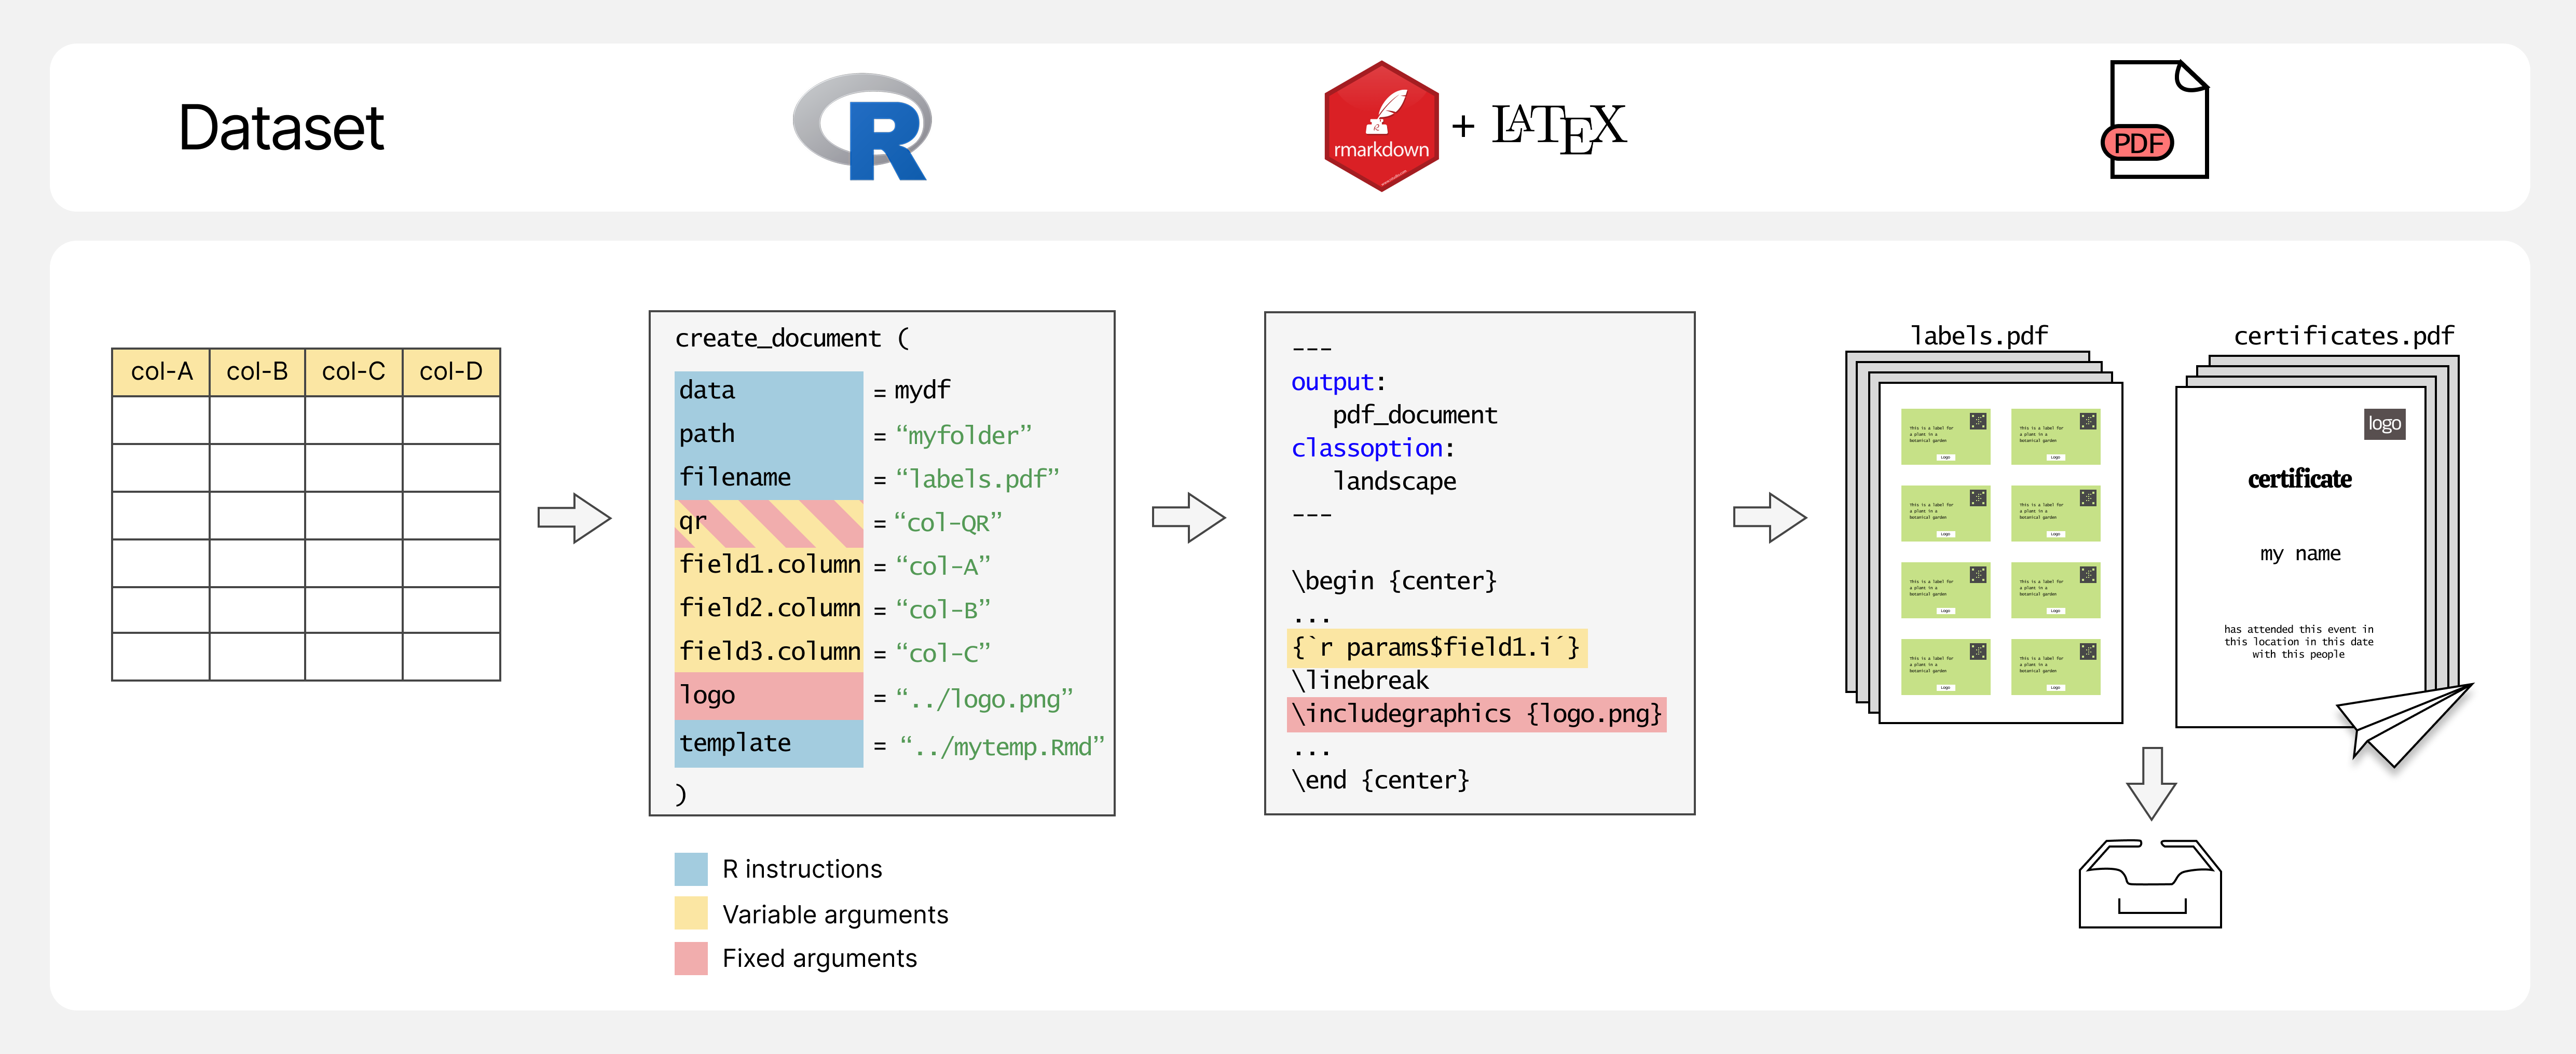
\includegraphics{figures/Fig1.png}
\caption{Figure 1. \texttt{labeleR} package workflow. Information stored
in a dataset passes through an R function into a parameterized
\texttt{RMarkdown} file using LaTeX syntax, and is then rendered as PDF.
\texttt{labeleR} functions accept three argument types: R instructions
which specify the dataset, paths to images or add custom templates (in
blue); fixed arguments, such as titles or subtitles (in red), and
variable arguments, linked to columns of the dataset (in yellow). Users
work directly on R to introduce the parameters, while \texttt{labeleR}
works in the background with markdown and latex to produce the results.
Output PDF documents can be automatically emailed to participants.}
\end{figure}

\subsubsection{Herbarium labels}\label{herbarium-labels}

Herbarium labels are one of the documents with more variable parameters.
Note that the \texttt{family.column} content will always be capitalized,
and the \texttt{taxon.column} one in italics, recommended to be used as
originally defined, while the rest ca be interchangeable. The QR can
stand for a free text (and therefore remain identical in all labels), or
be a column name, and the codes will be rendered with the individual
information of each row. Four different labels will fit in each of the
A4 pdf pages.

\begin{Shaded}
\begin{Highlighting}[]
\FunctionTok{create\_herbarium\_label}\NormalTok{(}
  \AttributeTok{data =}\NormalTok{ herbarium.table,}
  \AttributeTok{path =} \StringTok{"labeleR\_output"}\NormalTok{,}
  \AttributeTok{filename =} \StringTok{"herbarium\_labels"}\NormalTok{,}
  \AttributeTok{qr =} \StringTok{"QR\_code"}\NormalTok{,}
  \AttributeTok{title =}\StringTok{"Magical flora of the British Isles"}\NormalTok{ ,}
  \AttributeTok{subtitle =} \StringTok{"Project: Eliminating plant blindness in Hogwarts students"}\NormalTok{,}
  \AttributeTok{family.column =} \StringTok{"Family"}\NormalTok{,}
  \AttributeTok{taxon.column =} \StringTok{"Taxon"}\NormalTok{,}
  \AttributeTok{author.column =} \StringTok{"Author"}\NormalTok{,}
  \AttributeTok{det.column =} \StringTok{"det"}\NormalTok{,}
  \AttributeTok{date.det.column =} \StringTok{"Det\_date"}\NormalTok{,}
  \AttributeTok{location.column =} \StringTok{"Location"}\NormalTok{,}
  \AttributeTok{area.description.column =} \StringTok{"Area\_description"}\NormalTok{,}
  \AttributeTok{latitude.column =} \StringTok{"Latitude"}\NormalTok{,}
  \AttributeTok{longitude.column =} \StringTok{"Longitude"}\NormalTok{,}
  \AttributeTok{elevation.column =} \StringTok{"Elevation"}\NormalTok{,}
  \AttributeTok{field1.column =} \StringTok{"life\_form"}\NormalTok{,}
  \AttributeTok{field2.column =} \StringTok{"Observations"}\NormalTok{,}
  \AttributeTok{field3.column =} \StringTok{"Height"}\NormalTok{,}
  \AttributeTok{collector.column =} \StringTok{"Collector"}\NormalTok{,}
  \AttributeTok{collection.column =} \StringTok{"Collection\_number"}\NormalTok{,}
  \AttributeTok{assistants.column =} \StringTok{"Assistants"}\NormalTok{,}
  \AttributeTok{date.column =} \StringTok{"Date"}
\NormalTok{)}
\end{Highlighting}
\end{Shaded}

\subsubsection{Collection labels}\label{collection-labels}

They count with five variable parameters, which are not recommended to
be too long, along with the possibility of including a QR code (fixed or
variable) and an image (logo or picture). Field 1 will be always
capitalized, and Field 2 italicized. Any field can be left blank. The
user may manually fix the backgroud and text colors to their preference,
using HTML color codes. Eight different labels will fit in each of the
A4 pdf pages.

\begin{Shaded}
\begin{Highlighting}[]
\FunctionTok{create\_collection\_label}\NormalTok{(}
  \AttributeTok{data =}\NormalTok{ collection.table,}
  \AttributeTok{path =} \StringTok{"labeleR\_output"}\NormalTok{,}
  \AttributeTok{filename =} \StringTok{"labels"}\NormalTok{,}
  \AttributeTok{qr =} \StringTok{"QR\_code"}\NormalTok{,}
  \AttributeTok{field1.column =} \StringTok{"field1"}\NormalTok{,}
  \AttributeTok{field2.column =} \StringTok{"field2"}\NormalTok{,}
  \AttributeTok{field3.column =} \StringTok{"field3"}\NormalTok{,}
  \AttributeTok{field4.column =} \StringTok{"field6"}\NormalTok{,}
  \AttributeTok{field5.column =} \StringTok{"field7"}\NormalTok{,}
  \FunctionTok{system.file}\NormalTok{(}\StringTok{"rmarkdown/pictures/Hogwarts\_BnW.png"}\NormalTok{, }\AttributeTok{package =} \StringTok{"labeleR"}\NormalTok{),}
  \AttributeTok{bgcolor =} \StringTok{"D0ECC1"}\NormalTok{,  }\CommentTok{\#White is "FFFFFF",}
  \AttributeTok{textcolor =} \StringTok{"1E3F20"} \CommentTok{\#Black is "000000"}
\NormalTok{)}
\end{Highlighting}
\end{Shaded}

\subsubsection{Tiny labels}\label{tiny-labels}

This type of labels is a simplified version of the collection label,
including just five variable fields and the possibility of including a
QR code. It is recommended to write short texts in the variable
arguments and in the QR, as they might become difficult to read. 16
different labels will fit in each of the A4 pdf pages.

\begin{Shaded}
\begin{Highlighting}[]
\FunctionTok{create\_tiny\_label}\NormalTok{(}
  \AttributeTok{data =}\NormalTok{ tiny.table,}
  \AttributeTok{qr =} \StringTok{"QR\_code"}\NormalTok{,}
  \AttributeTok{path =} \StringTok{"labeleR\_output"}\NormalTok{,}
  \AttributeTok{filename =} \StringTok{"tinylabels"}\NormalTok{,}
  \AttributeTok{field1.column =}\StringTok{"field2"}\NormalTok{,}
  \AttributeTok{field2.column =}\StringTok{"field1"}\NormalTok{,}
  \AttributeTok{field3.column =}\StringTok{"field3"}\NormalTok{,}
  \AttributeTok{field4.column =}\StringTok{"field4"}\NormalTok{,}
  \AttributeTok{field5.column =}\StringTok{"field5"} 
\NormalTok{)}
\end{Highlighting}
\end{Shaded}

\begin{figure}
\centering
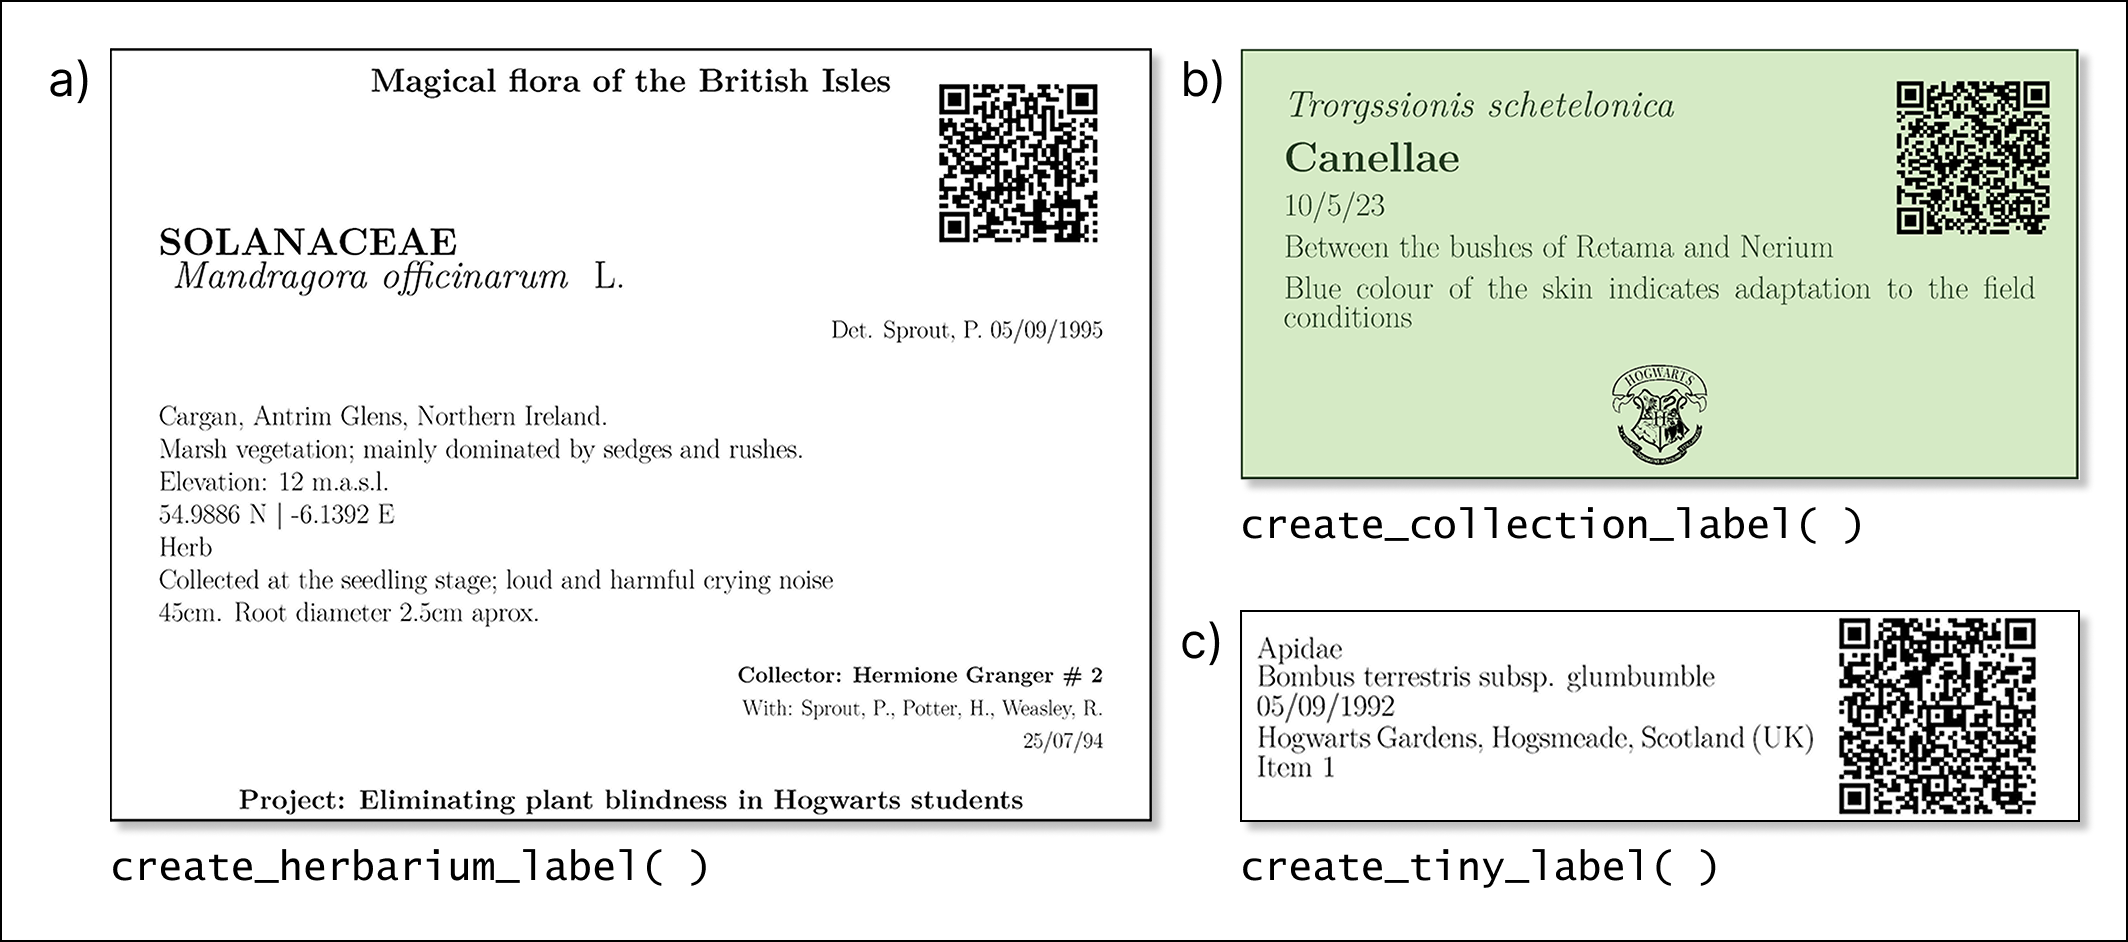
\includegraphics{figures/Fig2.png}
\caption{Figure 2. Examples of the outcomes from each label-related
function in \texttt{labeleR}. a) Herbarium label: for stored plant
vouchers; includes fixed fields (title, subtitle) and variable fields
(e.g.~taxon, date, coordinates, elevation). The family field is by
default capitalized and bold, and species name italic. Size: 4
labels/page. b) Collection label: includes variable fields (first field
in italics, second in bold), a customizable logo, font and background
colors. Size: 8/page. c) Tinylabel: a simplified collection label with
five fields. Size: 16/page. All three functions can include an optional
QR code.}
\end{figure}

\subsection{Documents for scientific
events}\label{documents-for-scientific-events}

Scientific events often host a high number of participants, and require
the creation of different documentation, such as abstract books,
personal identification badges and certificates for attendees and
participants. Bulk rendering significantly decreases the amount of time
invested in the creation of these documents. Moreover, to deliver
attendance and participation certificates automatically, those
\texttt{labeleR} functions allow users to automatically send individual
documents to email addresses stored in a column.

\subsubsection{Abstract book}\label{abstract-book}

Abstract books result in a single pdf document with multiple pages. Each
abstract will appear on a different page, following the same order as in
the dataframe rows. If other order of appearance is desired, it is
necessary to first arrange the columns in the original dataframe. Each
page will include four variable fields (title, author names,
affiliations and the abstract texts). The output document can include a
table of contents with the titles and page numbers of all abstracts.
Additionally, is possible to insert a custom front page that appearing
at the beginning of the document.

\begin{Shaded}
\begin{Highlighting}[]
\FunctionTok{create\_abstractbook}\NormalTok{(}
\AttributeTok{data=}\NormalTok{abstract.table,}
\AttributeTok{path =} \StringTok{"labeleR\_output"}\NormalTok{,}
\AttributeTok{filename =} \StringTok{"congress\_abstractbook"}\NormalTok{,}
\AttributeTok{title.column =} \StringTok{"abstract\_title"}\NormalTok{,}
\AttributeTok{authors.column =} \StringTok{"authors"}\NormalTok{,}
\AttributeTok{affiliation.column =} \StringTok{"affiliation"}\NormalTok{,}
\AttributeTok{text.column =} \StringTok{"abstract\_text"}\NormalTok{,}
\AttributeTok{title.cex =} \DecValTok{20}\NormalTok{,}
\AttributeTok{authors.cex =} \DecValTok{15}\NormalTok{,}
\AttributeTok{affiliations.cex =} \DecValTok{14}\NormalTok{,}
\AttributeTok{text.cex =} \DecValTok{12}\NormalTok{,}
\AttributeTok{frontpage =} \StringTok{"Congress\_frontpage.pdf"}
\NormalTok{)}
\end{Highlighting}
\end{Shaded}

\subsubsection{Badges}\label{badges}

Badges can be used for personal accreditation in congresses, courses,
meetings, etc. They have only two variable fields (name and
affiliation), and can include two top logos or images. Accreditation
badges include a dot line in the bottom for individual hand-edition once
printed.

\begin{Shaded}
\begin{Highlighting}[]
\FunctionTok{create\_badge}\NormalTok{(}
  \AttributeTok{data =}\NormalTok{ badges.table,}
  \AttributeTok{path =} \StringTok{"labeleR\_output"}\NormalTok{,}
  \AttributeTok{filename =} \StringTok{"badges"}\NormalTok{,}
  \AttributeTok{event =} \StringTok{"INTERNATIONAL CONFERENCE OF MUGGLEOLOGY"}\NormalTok{,}
  \AttributeTok{name.column =} \StringTok{"List"}\NormalTok{,}
  \AttributeTok{affiliation.column =} \StringTok{"Affiliation"}\NormalTok{,}
  \AttributeTok{rpic =} \FunctionTok{system.file}\NormalTok{(}\StringTok{"rmarkdown/pictures/Hogwartslogo.png"}\NormalTok{, }\AttributeTok{package =} \StringTok{"labeleR"}\NormalTok{),}
  \AttributeTok{lpic =} \FunctionTok{system.file}\NormalTok{(}\StringTok{"rmarkdown/pictures/MinMagic.png"}\NormalTok{, }\AttributeTok{package =} \StringTok{"labeleR"}\NormalTok{)}
\NormalTok{)}
\end{Highlighting}
\end{Shaded}

\paragraph{2.2.3. Attendance
certificates}\label{attendance-certificates}

Attendance certificates the only variable parameter is the name of the
attendees. It allows to include a signature as an image, implying that
the signer does not have to sign them individually. This certificate is
available both in English and Spanish.

\begin{Shaded}
\begin{Highlighting}[]
\FunctionTok{create\_attendance\_certificate}\NormalTok{(}
  \AttributeTok{data =}\NormalTok{ attendance.table,}
  \AttributeTok{path =} \StringTok{"labeleR\_output"}\NormalTok{,}
  \AttributeTok{filename =} \StringTok{"attendance\_certificates"}\NormalTok{,}
  \AttributeTok{language =} \StringTok{"English"}\NormalTok{ ,}
  \AttributeTok{name.column =} \StringTok{"Names"}\NormalTok{,}
  \AttributeTok{type =} \StringTok{"class"}\NormalTok{,}
  \AttributeTok{title =} \StringTok{"Potions (year 1992{-}1993)"}\NormalTok{,}
  \AttributeTok{date =} \StringTok{"23/06/1993"}\NormalTok{,}
  \AttributeTok{hours =} \StringTok{"200"}\NormalTok{,}
  \AttributeTok{freetext =} \StringTok{"taught by Professor S. Snape"}\NormalTok{,}
  \AttributeTok{signer =} \StringTok{"A.P.W.B. Dumbledore"}\NormalTok{,}
  \AttributeTok{signer.role =} \StringTok{"School Headmaster"}\NormalTok{,}
  \AttributeTok{rpic =} \FunctionTok{system.file}\NormalTok{(}\StringTok{"rmarkdown/pictures/Hogwartslogo.png"}\NormalTok{, }\AttributeTok{package =} \StringTok{"labeleR"}\NormalTok{),}
  \AttributeTok{lpic =} \FunctionTok{system.file}\NormalTok{(}\StringTok{"rmarkdown/pictures/Hogwartslogo.png"}\NormalTok{, }\AttributeTok{package =} \StringTok{"labeleR"}\NormalTok{),}
  \AttributeTok{signature.pic =} \FunctionTok{system.file}\NormalTok{(}\StringTok{"rmarkdown/pictures/dumbledore.png"}\NormalTok{, }\AttributeTok{package =} \StringTok{"labeleR"}\NormalTok{)}
\NormalTok{)}
\end{Highlighting}
\end{Shaded}

\subsubsection{Participation
certificates}\label{participation-certificates}

Participation certificates include multiple variable parameters (such as
speaker, affiliation, title, etc.). These documents can be rendered in
English and in Spanish.

\begin{Shaded}
\begin{Highlighting}[]
\FunctionTok{create\_participation\_certificate}\NormalTok{(}
  \AttributeTok{data =}\NormalTok{ participation.table,}
  \AttributeTok{path =} \StringTok{"labeleR\_output"}\NormalTok{,}
  \AttributeTok{filename =} \StringTok{"participation\_certificates"}\NormalTok{,}
  \AttributeTok{language =} \StringTok{"English"}\NormalTok{,}
  \AttributeTok{name.column =} \StringTok{"Name"}\NormalTok{,}
  \AttributeTok{affiliation.column =} \StringTok{"House"}\NormalTok{,}
  \AttributeTok{comm.type.column =} \StringTok{"Comm.type"}\NormalTok{,}
  \AttributeTok{title.column =} \StringTok{"Title"}\NormalTok{,}
  \AttributeTok{date.column =} \StringTok{"Date"}\NormalTok{,}
  \AttributeTok{type =} \StringTok{"online"}\NormalTok{,}
  \AttributeTok{event =} \StringTok{"seminar"}\NormalTok{,}
  \AttributeTok{freetext =} \StringTok{"organized by Hogwarts School of Magic and Wizardry"}\NormalTok{,}
  \AttributeTok{signer =} \StringTok{"A.P.W.B. Dumbledore"}\NormalTok{,}
  \AttributeTok{signer.role =} \StringTok{"School Headmaster"}\NormalTok{,}
  \AttributeTok{rpic =} \FunctionTok{system.file}\NormalTok{(}\StringTok{"rmarkdown/pictures/Hogwartslogo.png"}\NormalTok{, }\AttributeTok{package =} \StringTok{"labeleR"}\NormalTok{),}
  \AttributeTok{lpic =} \FunctionTok{system.file}\NormalTok{(}\StringTok{"rmarkdown/pictures/MinMagic.png"}\NormalTok{, }\AttributeTok{package =} \StringTok{"labeleR"}\NormalTok{),}
  \AttributeTok{signature.pic =} \FunctionTok{system.file}\NormalTok{(}\StringTok{"rmarkdown/pictures/dumbledore.png"}\NormalTok{, }\AttributeTok{package =} \StringTok{"labeleR"}\NormalTok{)}
\NormalTok{)}
\end{Highlighting}
\end{Shaded}

\begin{figure}
\centering
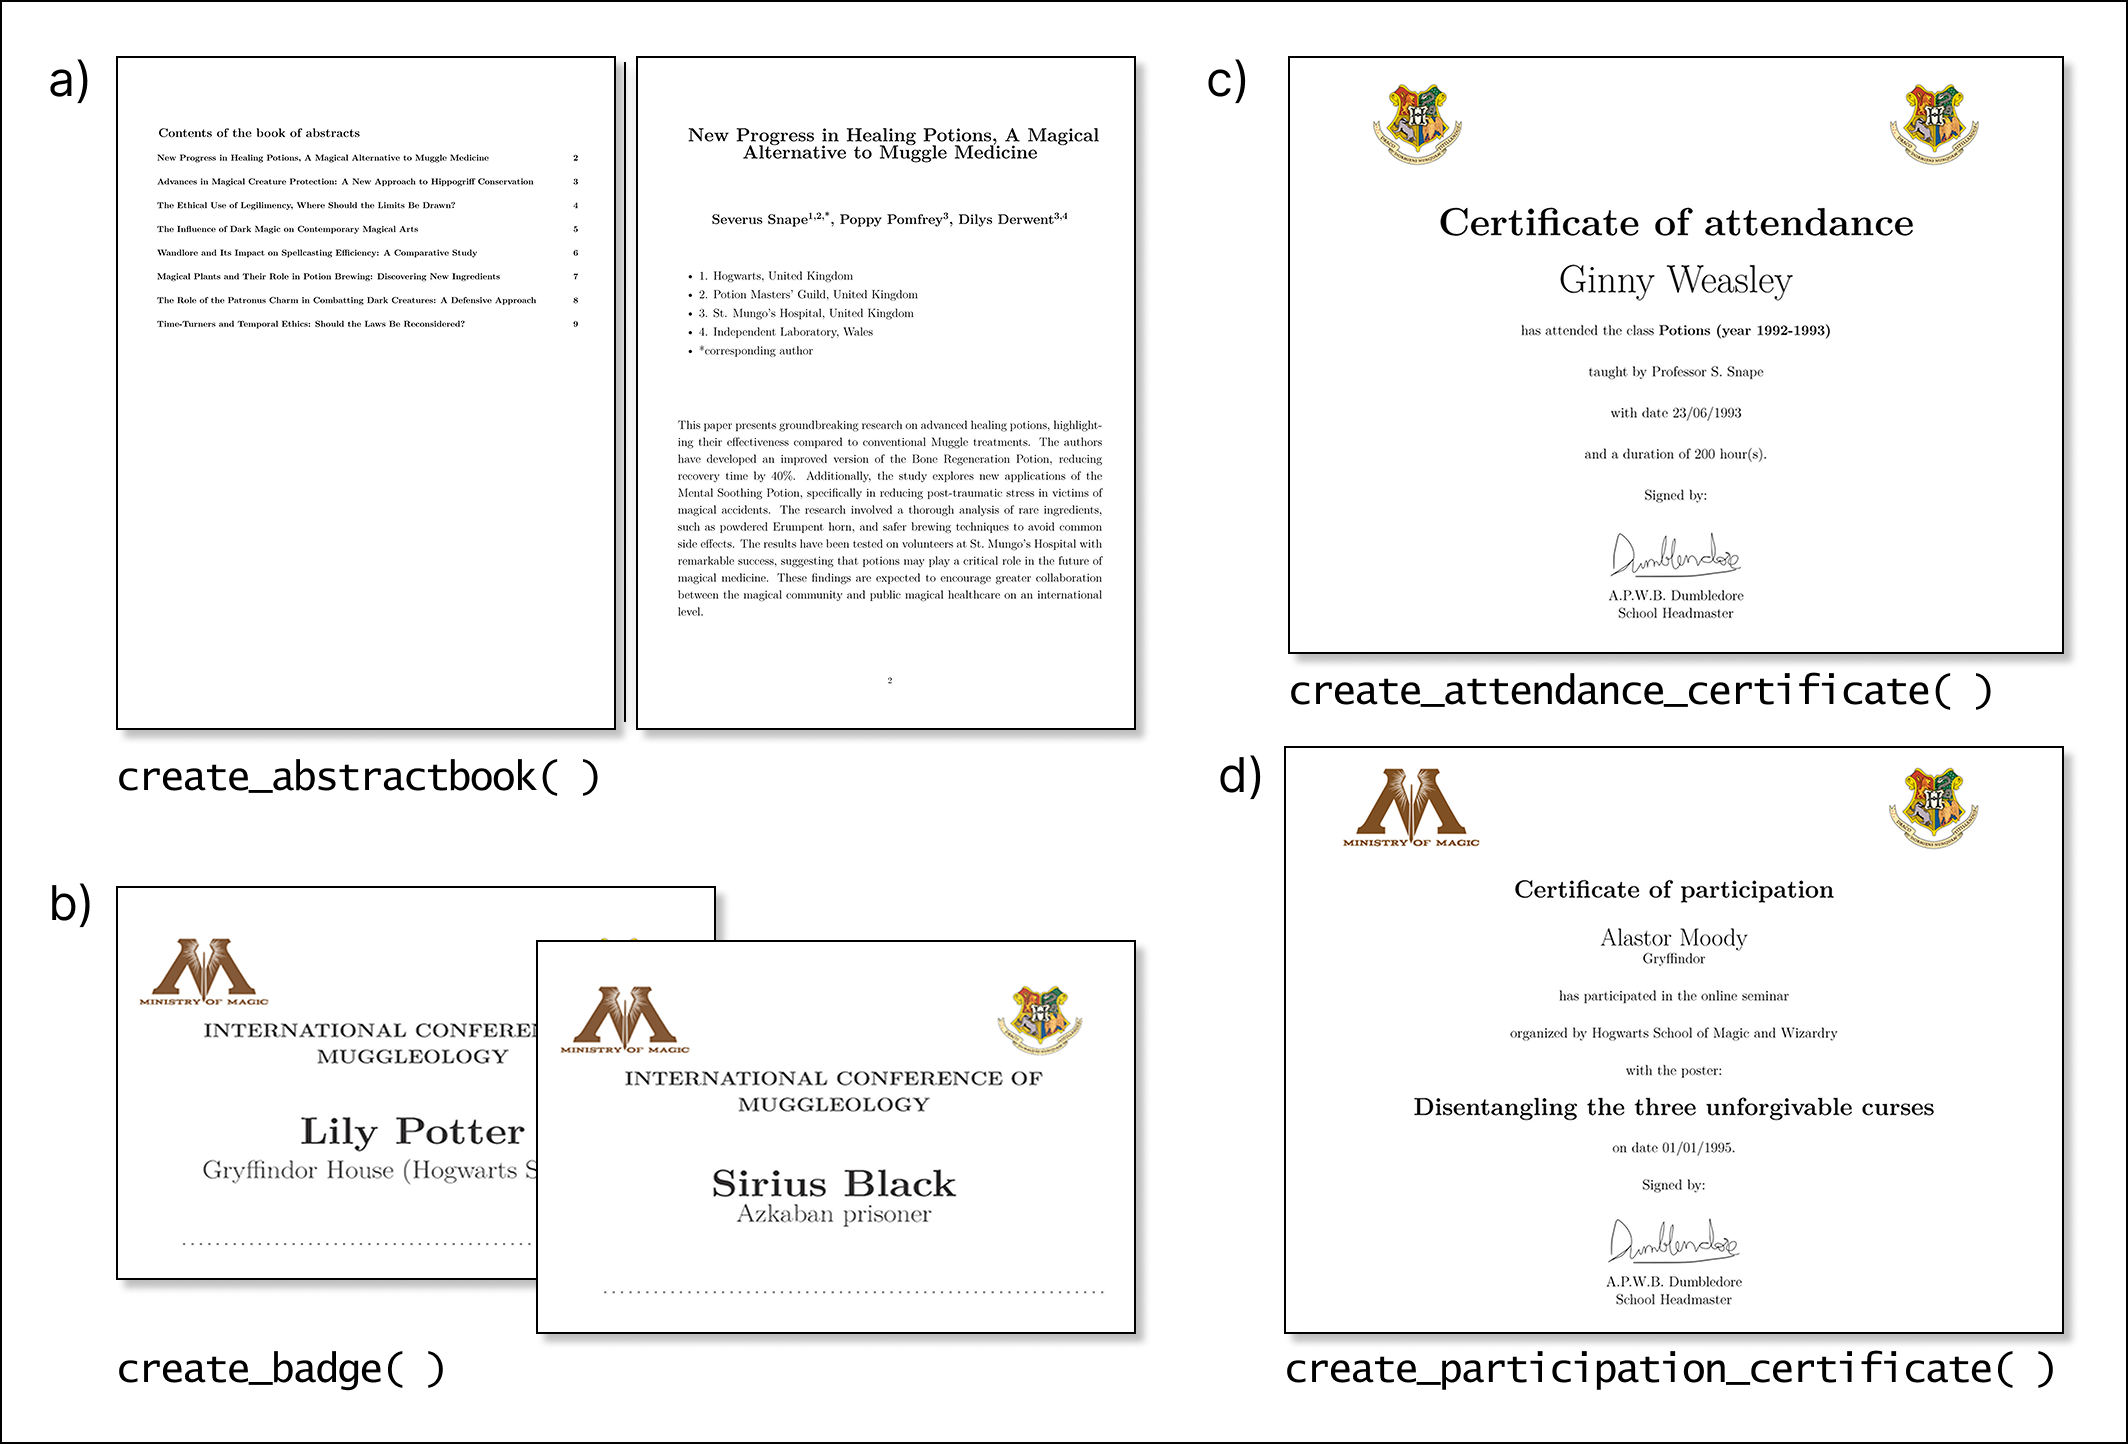
\includegraphics{figures/Fig3.png}
\caption{Figure 3. Examples of outcomes from each event-related function
in `labeleR. a) Abstract book: creates pages with title, authors,
affiliations and abstract (variable fields) and can include a table of
contents and front page. b) Badges: include name, affiliation, a fixed
field for the title, the option to add two images on top, and a dashed
line at the bottom for additional hand-written information. c)
Attendance certificate: attendee name is a variable field, while event
name, signer, and date are fixed fields. d) Participation certificate:
includes name, affiliation and title of the communication, and several
fixed fields. Both certificate functions allow two images on top, a
signature at the bottom, and offer Spanish and English templates.}
\end{figure}

\section{Customizable templates}\label{customizable-templates}

In case pictures look too big or small, it is possible to modify their
size in the template.

\section{Further applications}\label{further-applications}

The \texttt{labeleR} philosophy is quite simple: creating multiple
documents with a common design from a dataset containing the required
information. It offers a modular structure that allows for customization
and extension for new applications. For instance, the newly added
\texttt{create\_multichoice} function generates multichoice tests
randomizing the order of questions and possible answers from a given
table (question bank). New developments will happen in the GitHub
repository (\url{https://github.com/EcologyR/labeleR}) and eventually
pushed to CRAN. User feedback and code contributions are welcome in the
same repository to keep `labeleR as an open and dynamic tool.

\section{Acknowledgements}\label{acknowledgements}

This package has been developed collaboratively between Sevilla and
Madrid, with continuous feedback from colleagues in both locations. We
acknowledge their input, support and collaboration. We are especially
grateful to Manuel Molina for his ideas at `labeleR initial stages. We
would like to emphasize that the original idea has been built
horizontally among early career researchers. Our work has been possible
thanks to the support of the institutions and projects that employ us,
and especially by the software-developing workshop (Cádiz, La Muela,
2023) organized by AEET and funded by US-1381388 grant from Universidad
de Sevilla/Junta de Andalucía/FEDER-UE.

J.G.A. was supported by Next Generation EU Investigo contract
(URJC-AI-17) and ANTENNA Biodiversa+ and European Commission
(PCI2023-146022-2) postdoctoral contract. J.M.M. was supported by the
Comunidad de Madrid and Universidad Autónoma de Madrid doctoral grant
PEJ-2020-AI/AMB-17551 and research assistant contract
PIPF-2022/ECO-24251. F.R.-S. was supported by VI PPIT-US and grants
US-1381388 from Universidad de Sevilla/Junta de Andalucía/FEDER-UE and
CNS2022-135839 funded by MICIU/AEI/10.13039/501100011033 and by European
Union NextGenerationEU/PRTR. I.R.G. was supported by a doctoral grant at
Universidad Autónoma de Madrid and a postdoctoral position at
Universidad de Sevilla (CNS2022-135839).

\section*{References}\label{references}
\addcontentsline{toc}{section}{References}

\phantomsection\label{refs}
\begin{CSLReferences}{1}{0}
\bibitem[\citeproctext]{ref-rmarkdown}
Allaire, J., Xie, Y., Dervieux, C., McPherson, J., Luraschi, J., Ushey,
K., Atkins, A., et al. (2024). \emph{Rmarkdown: Dynamic documents for
r}. Retrieved from \url{https://github.com/rstudio/rmarkdown}

\bibitem[\citeproctext]{ref-brahms2025}
BRAHMS. (2025). Retrieved from
\url{https://herbaria.plants.ox.ac.uk/bol/brahms}

\bibitem[\citeproctext]{ref-entomolabels2022}
EntomoLabels. (2022). Retrieved from \url{https://labels.entomo.pl/}

\bibitem[\citeproctext]{ref-irisbg2024}
IrisBG. (2024). Retrieved from \url{https://www.irisbg.com}

\bibitem[\citeproctext]{ref-lichenlabler2025}
LichenLabler. (2025). Retrieved from \url{https://lichenportal.org/}

\bibitem[\citeproctext]{ref-elysia2019}
Pando, F., Lujano, C., \& Cezón, K. (2019). Elysia: Programa de gestión
de colecciones de biodiversidad (v.2.0). Digital.CSIC.
doi:\href{https://doi.org/10.20350/DIGITALCSIC/14520}{10.20350/DIGITALCSIC/14520}

\bibitem[\citeproctext]{ref-plabel2020}
pLabel. (2020). Retrieved from
\url{http://pfind.net/software/pLabel/index.html}

\bibitem[\citeproctext]{ref-herblabel}
Zhang, J., Zhu, H., Liu, J., \& Fischer, G. A. (2016). Principles behind
designing herbarium specimen labels and the {R} package 'herblabel'.
\emph{Biodiversity Science}, \emph{24}(12), 1345--1352.

\end{CSLReferences}

\end{document}
